\documentclass[10pt,letterpaper]{amspset}
\usepackage{fullpage}
\usepackage{gensymb}
\usepackage{graphicx}
\usepackage{tikz}
\usepackage{amsmath}
\usepackage{pgfplots}
\usepackage{amsthm}
\usepackage{amssymb}
\usepackage{pst-coil}
\usetikzlibrary{decorations.pathmorphing,patterns}
\pgfplotsset{compat=1.17}
\graphicspath{ {./images/} }
\notag


% info for header block in upper right hand corner
\name{Brady Lamson}
\class{MATH 1120 SPRING 2021}
\assignment{Applications of sinusoids Part II}
\duedate{Mar 14th}
\begin{document}

\problemlist{Applications of sinusoids Part II: 

Section 11.1: Problems 1--8}

\begin{problem}[1]
    The sounds we hear are made up of mechanical waves. The note 'A' above the note 'middle C' is a sound wave with ordinary frequency $f = 440Hz = 440 \frac{\text{cycles}}{\text{second}}$. Find a sinusoid which models this note, assuming that the amplitude is 1 and the phase shift is 0.
\end{problem}

\begin{solution}
    As always let's start with what we know. Our goal format will be as follows: 
    
    \[S(x) = A sin(\omega x + \phi) + \beta\]
    
    We know the amplitude is 1 and the phase shift is 0. There is also nothing in this problem that would imply a vertical shift at all. So that's 0 as well. So we have the following format:
    
    \[S(x) = sin(\omega x) \]
    
    Now we just calculate $\omega$. 
    
    \[\text{Ordinary Frequency} = \frac{\omega}{2\pi}\]
    \[440 = \frac{\omega}{2\pi}\]
    \[\omega = 880\pi\]
    
    Plug this back into S(x) and we're done.
    
    \[\boxed{ S(x) = sin(880\pi \cdot x)  }\]
\end{solution}


\begin{problem}[2]
    The voltage $V$ in an alternating current source has amplitude $220\sqrt{2}$ and ordinary frequency $f = 60$ Hertz. Find a sinusoid which models this voltage. Assume that the phase is 0. 
\end{problem}

\begin{solution}
    We are given multiple known values. All we really need to do is another quick conversion to find $\omega$ and we'll be done. 
    
    \[\text{Ordinary Frequency} = \frac{\omega}{2\pi}\]
    \[60 = \frac{\omega}{2\pi}\]
    \[\omega = 120\pi\]
    
    From here we can plug in our known values and we are done. Don't over-complicate this one. It's just here to get us used to these new units and how they relate to a sinusoidal format.
    
    \[\boxed{ S(t) = 220\sqrt{2} sin (120\pi \cdot t) }\]
\end{solution}


\pagebreak


\begin{problem}[3]
    A Ferris wheel has a \textbf{diameter of 135 meters} and makes \textbf{ one revolution (counter-clockwise) every thirty minutes}. The \textbf{lowest part of the wheel reaches ground level}, enabling passengers to simply walk on to, and off of, the ride. Find a sinusoid which models the height $h$ of the passenger above the ground in meters $t$ minutes after they board the wheel at \textbf{ground level}.
\end{problem}

\begin{solution}
    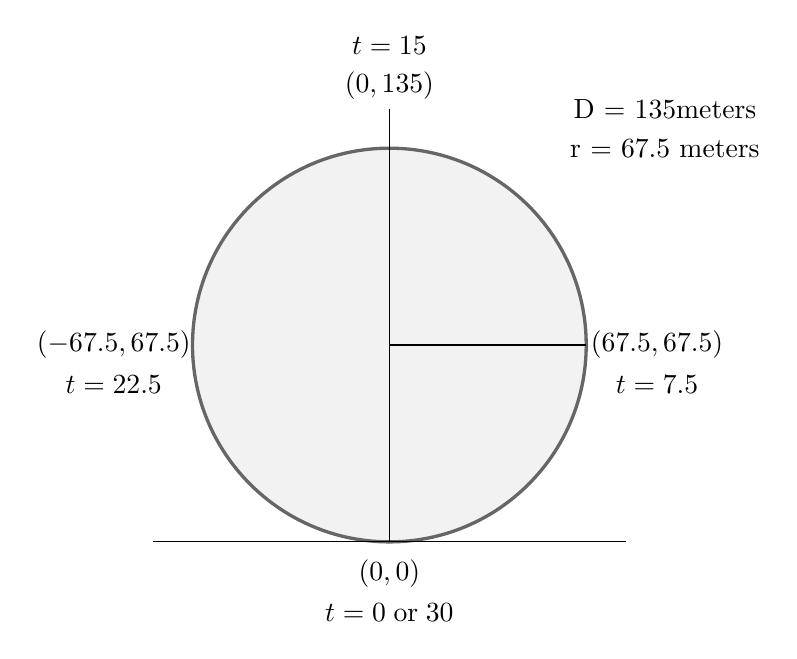
\begin{tikzpicture}
        %circle
            \filldraw[color=black!60, fill=black!5, very thick](0,0) circle (2.5);
        % lines
            \draw (-3,-2.5) -- (3,-2.5);
            \draw (0,3) -- (0,-2.5);
            \draw [thick ] (0,0) -- (2.5,0);
        %nodes
            \node[] at (3.4,0) {$(67.5, 67.5)$};
                \node[] at (3.4, -0.5) {$t = 7.5$};
            \node[] at (0, -2.9) {$(0, 0)$};
                \node at (0, -3.4) {$t = 0 \; \text{or} \; 30$};
            \node[] at (0, 3.3) {$(0, 135)$};
                \node[] at (0, 3.8) {$t = 15$};
            \node[] at (-3.5,0) {$(-67.5, 67.5)$};
                 \node[] at (-3.5, -0.5) {$t = 22.5$};
            \node[] at (3.5,3.0) {D = 135meters};
            \node[] at (3.5,2.5) {r = 67.5 meters};
    \end{tikzpicture}
    
    I always recommend starting with a diagram, writing out our desired sinusoidal format and exploring our given values.
    
    \[S(t) = A sin (\omega t + \phi) + \beta\]
    
    Now, upon inspection we know the following values: A, $\beta$ and with some calculations we will known $\omega$ as well. Remember, our period is one full rotation every thirty minutes.
    
    \[\omega = \frac{2\pi}{30} = \frac{\pi}{15}\]
    
    We know A because we know the diameter. The maximum amplitude is equal to the radius which in this case is $67.5$. As for $\beta$ we know that the wheel goes up to 135 meters and down to 0 meters. Since the wheel touches ground level at its lowest point we know that the wheel must also be vertically shifted up by its radius. So that is also $67.5$.
    
    The last thing we need to know is our phase shift. This is the weirdest part to wrap our head around. Let's plug in $S(t = 0)$ to calculate $\phi$ and then we'll make our final formula.
    
    \begin{align}
        S(t) = A sin (\frac{\pi}{15} \cdot t + \phi) + \beta \\
        S(0) = 67.5 sin (0 + \phi) + 67.5 &= 0 \\
        67.5 sin(\phi) = -67.5 \\
        sin(\phi) = -1 \\
        \phi = -\frac{\pi}{2} \; \text{or} \; + \frac{3\pi}{2}
    \end{align}
    
    \[\boxed{ S(t) = 67.5 \sin \left( \frac{\pi}{15} \cdot t - \frac{\pi}{2} \right) + 67.5  }\]
\end{solution}

\pagebreak


\begin{problem}[4]
    The x-coordinate of counter-clockwise motion on a circle of radius $r$ with angular frequency $\omega$ to be $x = r \cos(\omega t)$, where $t = 0$ corresponds to the point (r, 0). Suppose we are in the situation of Exercise 3 above. Find a sinusoid which models the horizontal displacement x of the passenger from the center of the wheel in meters t minutes after they board the wheel. Here we take $x(t) > 0$ to mean the passenger is to the right of the center, while $x(t) < 0$ means the passenger is to the left of the center.
\end{problem}

\begin{solution}
    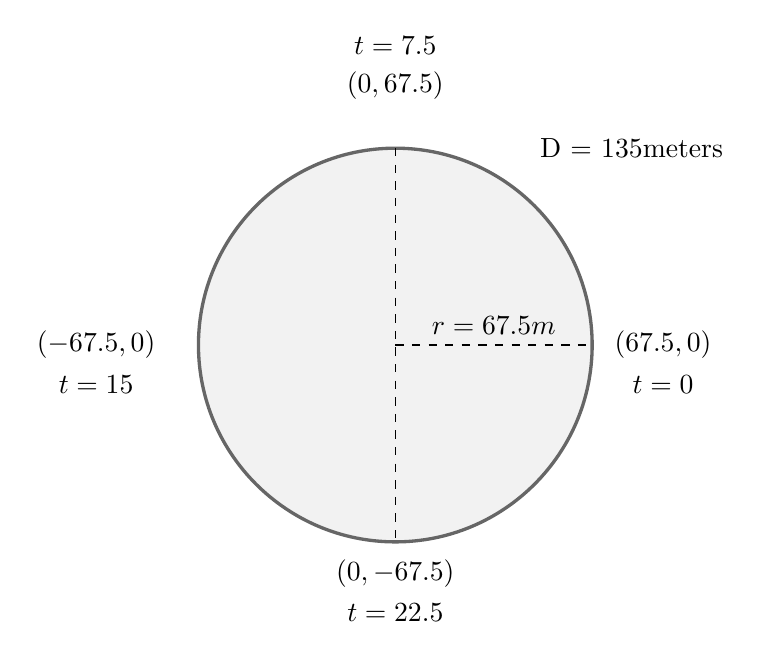
\begin{tikzpicture}
        %circle
            \filldraw[color=black!60, fill=black!5, very thick](0,0) circle (2.5);
        % lines
            \draw [dashed] (0,2.5) - - (0,-2.5);
            \draw [dashed] [thick ] (0,0) -- (2.5,0);
        %nodes
            \node[] at (3.4,0) {$(67.5, 0)$};
                \node[] at (3.4, -0.5) {$t = 0$};
            \node[] at (0, -2.9) {$(0, -67.5)$};
                \node at (0, -3.4) {$t = 22.5$};
            \node[] at (0, 3.3) {$(0, 67.5)$};
                \node[] at (0, 3.8) {$t = 7.5$};
            \node[] at (-3.8,0) {$(-67.5, 0)$};
                 \node[] at (-3.8, -0.5) {$t = 15$};
            \node[] at (3,2.5) {D = 135meters};
            \node[] at (1.25,0.25) {$r = 67.5m$ };
    \end{tikzpicture}
    
    So, for this problem we can thankfully reuse some of the information from the previous problem. Our period will still be the same, as will the radius. Our circle is different though, centered on $(0,0)$ now and our "starting point" is at $(r,0)$. So we're now working with a bit more of a traditional unit circle here. Due to the information provided we can also safely assume our $\beta$ value is 0. Let's get started. The best way to proceed is by working with $t = 0$ and recalculating $\phi$. I will also be using $r$ instead of the numerical value of it to make the work more coherent. 
    
    \[X(t) = r \cdot cos \left( \frac{\pi}{15} \cdot t + \phi \right)\]
    
    So, we know that at $t=0$ we're at $(r, 0)$. What this means is that $X(0) = r$ and $cos(0) = r$. If we think back to the normal unit circle the second thing I said there is true. $cos(0) = 1$ right? Same idea here. So, let's keep going.
    
    \begin{align}
    X(0) = r &= r \cdot cos \left( \frac{\pi}{15} \cdot 0 + \phi \right) \\
    r &= r \cdot cos \left(0 + \phi \right) \\
    \frac{r}{r} &= cos(\phi) \\
    1 &= cos(\phi) \\
    \phi &= 0 
    \end{align}
    
    \[\boxed{X(t) = 67.5 \cos \left( \frac{\pi}{15} \cdot t \right)} \]
    
    What you'll find is that my answer differs from that in the book ($\phi = -\frac{\pi}{2}$ there). That's because I am confident that the textbooks answer is incorrect. Let's quickly prove that then okay? Let's do the same work but plug $-\frac{\pi}{2}$ into our function.
    
    \begin{align}
    X(0) = r &= r \cdot cos \left( \frac{\pi}{15} \cdot 0 -\frac{\pi}{2} \right) \\
    r &= r \cdot cos \left(0 - \frac{\pi}{2} \right) \\
    \frac{r}{r} &= cos \left( -\frac{\pi}{2} \right) \\
    1 &= cos \left( -\frac{\pi}{2} \right) \\
    1 &\neq 0 
    \end{align}
    
    Due to this I can confidently state that the textbooks answer is wrong. 
\end{solution}


\pagebreak


\begin{problem}[5]
    In Exercise 52 in Section 10.1, we introduced the yo-yo trick ‘Around the World’ in which a yo-yo is thrown so it sweeps out a vertical circle. As in that exercise, suppose the yo-yo string is 28 inches and it completes one revolution in 3 seconds. If the closest the yo-yo ever gets to the ground is 2 inches, find a sinsuoid which models the height h of the yo-yo above the ground in inches t seconds after it leaves its lowest point. 
\end{problem}

\begin{solution}
        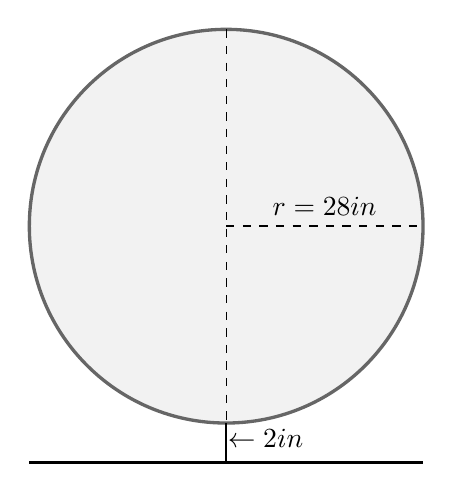
\begin{tikzpicture}
        %circle
            \filldraw[color=black!60, fill=black!5, very thick](0,0) circle (2.5);
        % lines
            \draw [dashed] (0,2.5) - - (0,-2.5);
            \draw [dashed] [thick ] (0,0) -- (2.5,0);
            \draw [thick] (0,-2.5) -- (0, -3.0);
            \draw [thick] (-2.5, -3) -- (2.5, -3); 
            \node[] at (1.25,0.25) {$r = 28in$ };
            \node[] at (0.5,-2.7) {$\leftarrow 2in$};
    \end{tikzpicture}

    So, based on the information given we know a few things. For one, since the yo-yo only ever gets 2 inches from the ground we know we have a vertical shift of $r + 2$, or $\beta = 30$ inches. \medskip
    
    We also know that since the radius itself is $28$ inches that we have an amplitude of 28. We also know that our starting point is at $(0,r)$ instead of $(r,0)$ so we'll need to shift our sinusoid by $-\frac{\pi}{2}$. \medskip 
    
    Lastly we just need our period which can solve for quickly. One revolution is completed in 3 seconds so we can say the period is $\frac{2\pi}{3sec}$ or just $\frac{2\pi}{3}$. From that we have our answer! 
    
    \[\boxed{S(x) = 28 sin \left( \frac{2\pi}{3} \cdot x - \frac{\pi}{2} \right) + 30 } \]
\end{solution}


\pagebreak


\begin{problem}[6]
    Suppose an object weighing 10 pounds is suspended from the ceiling by a spring which stretches 2 feet to its equilibrium position when the object is attached. \medskip
    
    (a) Find the spring constant $k$ in $\frac{\text{lbs}}{\text{ft}}$ and the mass of the object in slugs. \medskip
    
    (b) Find the equation of motion of the object if it is released from 1 foot below the equilibrium position from rest. When is the first time the object passes through the equilibrium position? In which direction is it heading? \medskip
    
    (c) Find the equation of motion of the object if it is released from 6 inches above the equilibrium position with a downward velocity of 2 feet per second. Find when the object passes through the equilibrium position heading downwards for the third time.
\end{problem}

\begin{solution}[(a)]
    This bits nice and simple, we just need to do some simple unit conversions. Our weights mass is 10lbs and it stretches our spring by 2 feet. 
    
    \[k = \frac{10}{2} \; \; \; \boxed{k = 5 \frac{ \text{lbs} }{ \text{ft} }  }\]
    \[1 \text{slug} = 32 \frac{\text{lbs} }{1 \text{ft} }\]
    \[m = \frac{10}{32} = \boxed{ \frac{5}{16} \text{slugs} }\] 
\end{solution}

\begin{solution}[(b)]

    First, as always we need to make a diagram. \medskip

    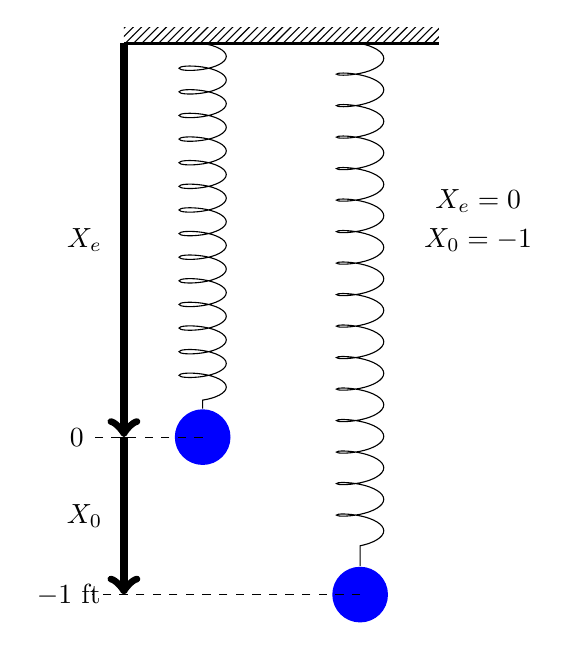
\begin{tikzpicture}
        % Weights    
            \node[circle,fill=blue,inner sep=2.5mm] (a) at (0,0) {};
            \node[circle,fill=blue,inner sep=2.5mm] (b) at (2,-2) {};
        % Coil specs
            \draw[decoration={aspect=0.3, segment length=3mm, amplitude=3mm,coil},decorate] (0,5) -- (a); 
            \draw[decoration={aspect=0.3, segment length=4mm, amplitude=3mm,coil},decorate] (2,5) -- (b);
        % Additional nodes for detail
            % First arrow
                \draw [->, line width = 3pt] (-1, 5) -- (-1, 0);
                \node[] at (-1.5, 2.5) {$X_e$};
                \node[] at (-1.6, 0) {$0$};
                \draw[dashed] (0,0) -- (-1.4,0);
            % Second arrow
                \draw [->, line width = 3pt] (-1, 0) -- (-1, -2);
                \draw[dashed] (2,-2) -- (-1.4,-2);
                \node[] at (-1.5, -1) {$X_0$};
                \node[] at (-1.7, -2) {$-1$ ft};
        \fill [pattern = north east lines] (-1,5) rectangle (3,5.2);
        \draw[thick] (-1,5) -- (3,5);
        \node[] at (3.5,3) {$X_e = 0$};
        \node[] at (3.5,2.5) {$X_0 = -1$};
    \end{tikzpicture}
    
    Now we need to list off our givens. 
    
    \begin{align}
        \text{mass} &= \frac{5}{16} \text{slugs} \\
        V_0 &= 0 \frac{ \text{ft} }{ \text{s} } \\
        k &= 5 \frac{ \text{lbs} }{ \text{ft} } \\
    \end{align}
    
    \pagebreak
    
    Our sinusoid will have the following format:
    
    \[X(t) = a \cdot \sin(\omega \cdot t + \phi)\]
    \[\omega = \sqrt{ \frac{k}{m} }\]
    \[A = \sqrt{ x_0^2 + \left( \frac{v_0}{\omega} \right)^2 }\]
    \[A \sin (\phi) = x_0\]
    
    First we solve for $\omega$.
    
    \[\omega = \sqrt{ \frac{5}{ \frac{5}{16} } }\]
    \[\omega = \sqrt{16} = \pm 4\]
    
    Now solve for A.
    
    \[A = \sqrt{-1^2 + \left( \frac{0}{4} \right)^2}\]
    \[A = 1\]
    
    Now we solve for $\phi$.
    
    \[1 \cdot \sin(\phi) = x_0\]
    \[sin(\phi) = -1\]
    \[\phi = \frac{3\pi}{2}\]
    
    Now we have our full formula.
    
    \[\boxed{X(t) = 1 \cdot \sin(4t + \frac{3\pi}{2})}\]
    
    Finally we just need to solve for when $X(t) = 0$. Why 0? Well, remember, I defined our equilibrium point as 0! 
    
    \[X(t) = 0 = \sin(4t + \frac{3\pi}{2})\]
    
    We know that $sin(\theta) = 0$ when $\theta = 0, \pi, 2\pi$ and so on. Since $\frac{3\pi}{2}$ is greater than the first two options there we will need to use $2\pi$ here. We can set $4t + \frac{3\pi}{2} = 2\pi$.
    
    \[4t + \frac{3\pi}{2} = 2\pi\]
    \[4t = \frac{4\pi}{2} - \frac{3\pi}{2}\]
    \[4t = \frac{\pi}{2}\]
    \[\boxed{ t = \frac{\pi}{8} \; \text{seconds} }\]
\end{solution}

\pagebreak

\begin{problem}[6c]
    Find the equation of motion of the object if it is released from 6 inches above the equilibrium position with a downward velocity of 2 feet per second. Find when the object passes through the equilibrium position heading downwards for the third time.
\end{problem}

\begin{solution}
    Alright, so we can reuse a lot of our information here. The values that change are $x_0$ and $v_0$. I'll speed through this a bit faster so check part b if you need to clarify some steps.
    
    
    \begin{align}
        x_0 = \frac{1}{2} \\
        v_0 = 2 \frac{ft}{s} \\
        A = \sqrt{\left( \frac{1}{2} \right)^2 + \left( \frac{2}{4} \right)^2 } \\
        A = \sqrt{\frac{1}{2}} \\
        A = \frac{\sqrt{2}}{2}
    \end{align}
    
    \begin{align}
        A \sin(\phi) = x_0 \\ 
        \frac{\sqrt{2}}{2} \sin(\phi) = \frac{1}{2} \\
        sin(\phi) = \frac{\sqrt{2}}{2} \\
        \phi = \frac{\pi}{4}, \frac{3\pi}{4}, \frac{5\pi}{4}, ...
    \end{align}
    
    Now, we need to solve for when we hit $x_e$ for the third time going downward. We know that $sin(\theta) = 0$ when $\theta = 0, \pi, 2\pi, 3\pi, 4\pi, 5\pi$ and so on. We also know that with each $\pi$ we'll be alternating between down and upwards movement. We also know that we can't have $\theta = 0$ due to the addition happening with $\phi$. Therefore we can say that $\pi$ will be going down, $2\pi$ will go up and so on. So therefore, $5\pi$ will be the value of $\theta$ when we hit $x_e$ going down the third time. Finally we can wrap this up.
    
    \[X(t) = \frac{\sqrt{2}}{2} \sin \left( 4t + \frac{\pi}{4} \right) \]
    \[4t + \frac{\pi}{4} = 5\pi\]
    \[4t = \frac{19\pi}{4}\]
    \[\boxed{t = \frac{19\pi}{16} \; \text{seconds}}\]
\end{solution}
\end{document}